
% controlled-assessments.tex - Our first LaTeX example!

%%%%%%%%%%%%%%%%%%%%%%%%%%%%%%%%%%%%%%%%%
% Beamer Presentation
% LaTeX Template
% Version 1.0 (10/11/12)
%
% This template has been downloaded from:
% http://www.LaTeXTemplates.com
%
% License:
% CC BY-NC-SA 3.0 (http://creativecommons.org/licenses/by-nc-sa/3.0/)
%
%%%%%%%%%%%%%%%%%%%%%%%%%%%%%%%%%%%%%%%%%

%----------------------------------------------------------------------------------------
%	PACKAGES AND THEMES
%----------------------------------------------------------------------------------------

\documentclass{beamer}
\mode<presentation> {

% The Beamer class comes with a number of default slide themes
% which change the colors and layouts of slides. Below this is a list
% of all the themes, uncomment each in turn to see what they look like.

%\usetheme{default}
%\usetheme{AnnArbor}
%\usetheme{Antibes}
%\usetheme{Bergen}
%\usetheme{Berkeley}
%\usetheme{Berlin}
%\usetheme{Boadilla}
%\usetheme{CambridgeUS}
%\usetheme{Copenhagen}
%\usetheme{Darmstadt}
%\usetheme{Dresden}
%\usetheme{Frankfurt}
%\usetheme{Goettingen}
%\usetheme{Hannover}
%\usetheme{Ilmenau}
%\usetheme{JuanLesPins}
%\usetheme{Luebeck}
\usetheme{Madrid}
%\usetheme{Malmoe}
%\usetheme{Marburg}
%\usetheme{Montpellier}
%\usetheme{PaloAlto}
%\usetheme{Pittsburgh}
%\usetheme{Rochester}
%\usetheme{Singapore}
%\usetheme{Szeged}
%\usetheme{Warsaw}

% As well as themes, the Beamer class has a number of color themes
% for any slide theme. Uncomment each of these in turn to see how it
% changes the colors of your current slide theme.
\definecolor{mypurplish}{rgb}{0.3, 0.12, 0.4}
%\usecolortheme{albatross}
%\usecolortheme{beaver}
%\usecolortheme{beetle}
%\usecolortheme{crane}
%\usecolortheme{dolphin}
%\usecolortheme{dove}
%\usecolortheme{fly}
%\usecolortheme{lily}
%\usecolortheme{orchid}
%\usecolortheme{rose}
%\usecolortheme{seagull}
%\usecolortheme{seahorse}
%\usecolortheme{spruce}
%\usecolortheme{whale}
%\usecolortheme{wolverine}
\usecolortheme[named=mypurplish]{structure}
%\setbeamertemplate{footline} % To remove the footer line in all slides uncomment this line
%\setbeamertemplate{footline}[page number] % To replace the footer line in all slides with a simple slide count uncomment this line

%\setbeamertemplate{navigation symbols}{} % To remove the navigation symbols from the bottom of all slides uncomment this line
}
\usepackage{graphicx} % Allows including images
\usepackage{booktabs} % Allows the use of \toprule, \midrule and \bottomrule in tables
\usepackage{tikz}



\newcommand\RBox[1]{%
  \tikz\node[draw,rounded corners,align=center,] {#1};%
}  
\usepackage{color}
\usepackage{listings}
\usepackage{setspace}

\usepackage[framemethod=tikz]{mdframed}



\definecolor{Code}{rgb}{0,0,0}
\definecolor{Decorators}{rgb}{0.2,0.2,0.2}
\definecolor{Numbers}{rgb}{0.5,0,0}
\definecolor{MatchingBrackets}{rgb}{0.25,0.5,0.5}
\definecolor{Keywords}{rgb}{0,0,1}
\definecolor{self}{rgb}{1,0,0}
\definecolor{Strings}{rgb}{0,0.63,0}
\definecolor{Comments}{rgb}{0,0.63,1}
\definecolor{Backquotes}{rgb}{0,0.2,0}
\definecolor{Classname}{rgb}{0,0,1}
\definecolor{FunctionName}{rgb}{1,0,1}
\definecolor{Operators}{rgb}{0,0,0}
\definecolor{Background}{rgb}{0.95,0.95,0.95}


            
\lstset{
numbers=left,
numberstyle=\footnotesize,
numbersep=1em,
xleftmargin=1em,
framextopmargin=2em,
framexbottommargin=2em,
showspaces=false,
showtabs=false,
showstringspaces=false,
frame=l,
tabsize=4,
breaklines=true,
postbreak=\raisebox{0ex}[0ex][0ex]{\ensuremath{\color{red}\hookrightarrow\space}},
% Basic
basicstyle=\ttfamily\small\setstretch{1},
backgroundcolor=\color{Background},
language=Python,
% Comments
commentstyle=\color{Comments},
% Strings
stringstyle=\color{Strings},
morecomment=[s][\color{Strings}]{"""}{"""},
morecomment=[s][\color{Strings}]{'''}{'''},
% keywords
morekeywords={import,from,class,def,for,while,if,is,in,elif,else,not,and,or,print,break,continue,return,True,False,None,access,as,,del,except,exec,finally,global,import,lambda,pass,print,raise,try,assert},
keywordstyle={\color{Keywords}\bfseries},
% additional keywords
morekeywords={[2]@invariant},
keywordstyle={[2]\color{Decorators}\slshape},
emph={self},
emphstyle={\color{self}\slshape},
%
}{}

\title[GUIs]{Python Graphical Toolkits}
\author[Dave Ames]{Dave Ames}
\institute[CAS]{Computing At School}


\begin{document}

{
  \usebackgroundtemplate{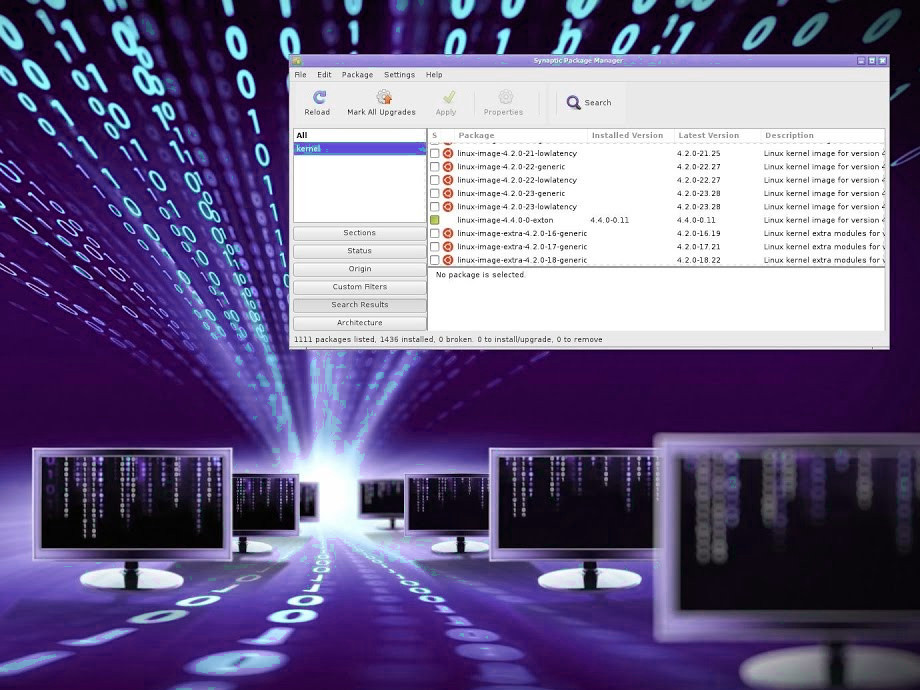
\includegraphics[width=1.0\paperwidth]{background2.jpg}}
  \begin{frame}[plain]
    \vspace{2cm}
    \centering
\begin{mdframed}[tikzsetting={draw=mypurplish,fill=white,fill opacity=0.8,
               line width=3pt},backgroundcolor=none,leftmargin=20,
               rightmargin=20,innertopmargin=8pt,roundcorner=15pt]
               {\huge \inserttitle} \\
               \insertauthor  \hspace{0.4cm}  (\insertinstitute) \hspace{0.3cm}  \insertdate \\
               \href{mailto:dave.ames@computingatschool.org.uk}{E: dave.ames@computingatschool.org.uk} \hspace{0.2cm}
               \href{http://twitter.com/davidames}{T: @DavidAmes}
               
             \end{mdframed}
\end{frame}
}




\section{Main part}



\begin{frame}
\frametitle{Installing Modules Using Pip}
\subsection{Installing Modules Using Pip}

\pause
\textbf{Pros}
\begin{itemize}
\pause
\item Comes as standard with modern versions of Python (provided it's installed correctly)
\pause
\item Deals with dependencies
\pause
\item At least 100 000 packages to choose from
\end{itemize}

\pause
\textbf{Cons}
\begin{itemize}
\pause
\item Requires administrator rights
\pause
\item Requires the command line
\pause
\item Standard way is not to install to main Python install, but to use a venv (Virtual ENVironment)
\end{itemize}

\end{frame}

\begin{frame}
\frametitle{How to use Pip}
\subsection{How to use Pip}

\pause
\textbf{Two main ways to use:} \\
\pause
\textbf{Way one:}
\begin{enumerate}
\pause
\item From the command line type: \lstinline{pip install requests}
\pause
\item You may need to do this in a console that has been given administrator rights
\pause
\item If you are on Linux using Python 3 then you may need to type \lstinline{pip3 install requests} instead
\end{enumerate}
\pause
\textbf{Way two:}
\begin{enumerate}
\pause
\item From the command line type either \lstinline{python} or \lstinline{python3} to check the python interpreter is
  available
\pause
\item Once python has started type \lstinline{exit()} to close the python shell again
\pause
\item Now type \lstinline{python -m pip install sqlalchemy} or use \lstinline{python3 -m pip install sqlalchemy}
     
\end{enumerate}

\pause
For some of the libraries we are going to use today, you can just use pip install to install them!

\end{frame}



\end{document}

%%% Local Variables:
%%% mode: latex
%%% TeX-master: t
%%% End:
